\documentclass[12pt,titlepage]{article}
\usepackage[margin=1.25in]{geometry}
\usepackage{graphicx,amsmath,minted}

%% Variables definition
\newcommand{\vSubject}{Advanced Database}
\newcommand{\vSubtitle}{Pivot}
\newcommand{\vName}{Dicha Zelianivan Arkana}
\newcommand{\vNIM}{2241720002}
\newcommand{\vClass}{2i}
\newcommand{\vDepartment}{Information Technology}
\newcommand{\vStudyProgram}{D4 Informatics Engineering}

%% [START] Tikz related stuff
\usepackage{tikz}
\usetikzlibrary{svg.path,calc,shapes.geometric,shapes.misc}
\tikzstyle{terminator} = [rectangle, draw, text centered, rounded corners = 1em, minimum height=2em]
\tikzstyle{preparation} = [chamfered rectangle, chamfered rectangle sep=0.75em, draw, text centered, minimum height = 2em]
\tikzstyle{process} = [rectangle, draw, text centered, minimum height=2em]
\tikzstyle{decision} = [diamond, aspect=2, draw, text centered, minimum height=2em]
\tikzstyle{data}=[trapezium, draw, text centered, trapezium left angle=60, trapezium right angle=120, minimum height=2em]
\tikzstyle{connector} = [line width=0.25mm,->]
%% [END] Tikz related stuff

%% [START] Fancy header related stuff
\usepackage{fancyhdr}
\pagestyle{fancy}
\setlength{\headheight}{15pt} % compensate fancyhdr style
\fancyhead{}
\fancyfoot{}
\fancyfoot[L]{\thepage}
\fancyfoot[R]{\textit{\vSubject - \vSubtitle}}
\renewcommand{\footrulewidth}{0.4pt}% default is 0pt, overline for footer
%% [END] Fancy header related stuff

%% [START] Custom tabular command related stuff
\usepackage{tabularx}
\newcommand{\details}[2]{
    #1 & #2  \\
}
%% [END] Custom tabular command related stuff

%% [START] Figure related stuff
\newcommand{\image}[3][1]{
    \begin{figure}[h]
        \centering
        \includegraphics[#1]{#2}
        \caption{#3}
        \label{#3}
    \end{figure}
}
%% [END] Figure related stuff

\begin{document}
\begin{titlepage}
    \centering
    \vfill
    {\bfseries\LARGE
        \vSubject\\
        \vskip0.25cm
        \vSubtitle
    }
    \vfill
    
\includegraphics[width=6cm]{images/polinema-logo.png}
    \vfill
    {
        \textbf{Name}\\
        \vName\\
        \vskip0.5cm
        \textbf{NIM}\\
        \vNIM\\
        \vskip0.5cm
        \textbf{Class}\\
        \vClass\\
        \vskip0.5cm
        \textbf{Department}\\
        \vDepartment\\
        \vskip0.5cm
        \textbf{Study Program}\\
        \vStudyProgram
    }
\end{titlepage}

\section{Practicum}

\begin{enumerate}
    \item {
        Dari view \texttt{Sales.CustGroups} yang sudah dibuat, buatlah sebuah query SELECT untuk
        menampilkan kolom \texttt{custid}, \texttt{custgroup}, dan \texttt{country}.

        \begin{minted}[autogobble,fontsize=\small]{sql}
            SELECT custid, custgroup, country
            FROM Sales.CustGroups;
        \end{minted}

        \begin{center}
            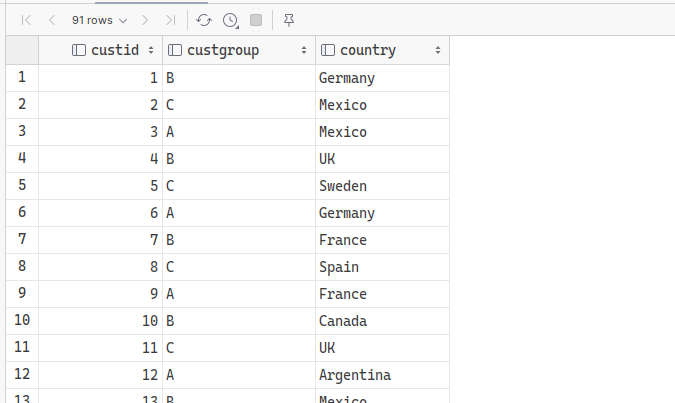
\includegraphics[width=0.8\textwidth]{./images/1.png}
        \end{center}
    }
    \item {
        Modifikasilah kode T-SQL dari langkah no 3 di atas dengan menampilkan kolom country,
        lalu dengan menggunakan operator PIVOT, tambahkan 3 kolom tambahan yang berisi banyaknya
        customer dalam masing-masing grup (A, B, \& C)

        \begin{minted}[autogobble,fontsize=\small]{sql}
            SELECT country, A, B, C
            FROM (
                SELECT custid, custgroup, country
                FROM Sales.CustGroups
            ) AS SourceTable
            PIVOT (
                COUNT(custid)
                FOR custgroup IN (A, B, C)
            ) AS PivotTable;
        \end{minted}

        \begin{center}
            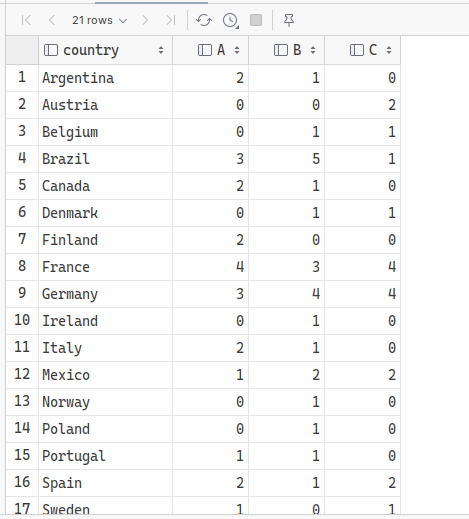
\includegraphics[width=0.8\textwidth]{./images/2.png}
        \end{center}
    }
    \pagebreak
    \item {
        Salinlah statement SELECT dari Soal no 2 di atas, lalu jalankan kembali. Apakah hasil
        query ini sama dengan hasil pada Praktikum Bagian 1 no 4 di atas? Apakah jumlah baris yang
        dihasilkan sama persis?

        \begin{center}
            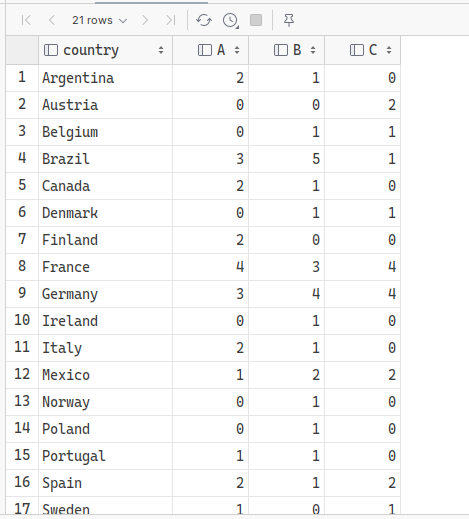
\includegraphics[width=0.8\textwidth]{./images/3.png}
        \end{center}

        Hasil query ini sama dengan hasil pada Praktikum Bagian 1 no 4 di atas. Jumlah baris yang
        dihasilkan sama persis. Hal ini dikarenakan perintah alter digunakan untuk menambahkan kolom
        namun kita tidak melakukan SELECT terhadap kolom tersebut.
    }
    \pagebreak
    \item {
        Modifikasi statement SELECT untuk menambahkan kolom city dan contactname!

        \begin{minted}[autogobble,fontsize=\small]{sql}
            SELECT country, city, contactname, A, B, C
            FROM (
                SELECT custid, custgroup, country, city, contactname
                FROM Sales.CustGroups
            ) AS SourceTable
            PIVOT (
                COUNT(custid)
                FOR custgroup IN (A, B, C)
            ) AS PivotTable;
        \end{minted}

        \begin{center}
            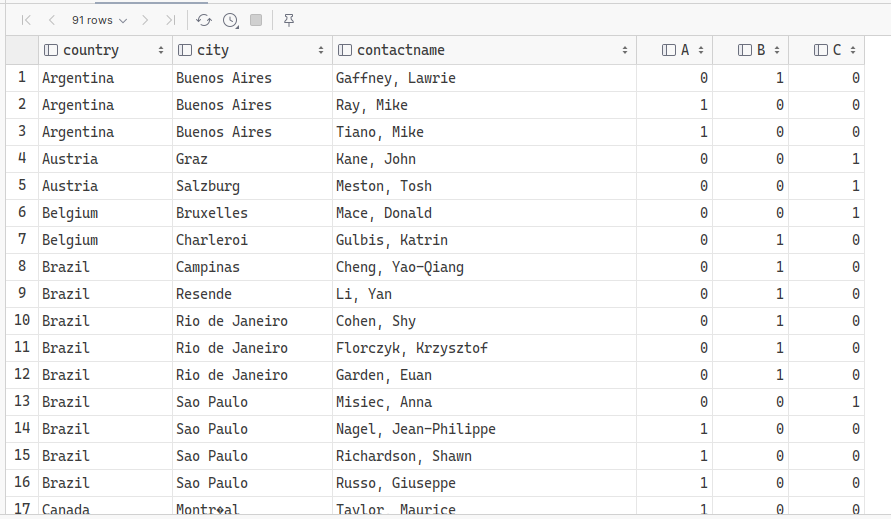
\includegraphics[width=0.8\textwidth]{./images/4.png}
        \end{center}
    }
    \pagebreak
    \item {
        Buatlah sebuah CTE bernama PivotCustGroups yang mendapatkan kolom custid,
        country, dan custgroup dari view Sales.CustGroups. Kemudian, buatlah sebuah query SELECT
        terhadap CTE tersebut dan gunakan operator PIVOT, seperti halnya dalam query SELECT pada
        Praktikum Bagian sebelumnya.

        \begin{minted}[autogobble,fontsize=\small]{sql}
            WITH PivotCustGroups AS (
                SELECT custid, custgroup, country
                FROM Sales.CustGroups
            )
            SELECT country, A, B, C
            FROM PivotCustGroups
            PIVOT (
                COUNT(custid)
                FOR custgroup IN (A, B, C)
            ) AS PivotTable;
        \end{minted}

        \begin{center}
            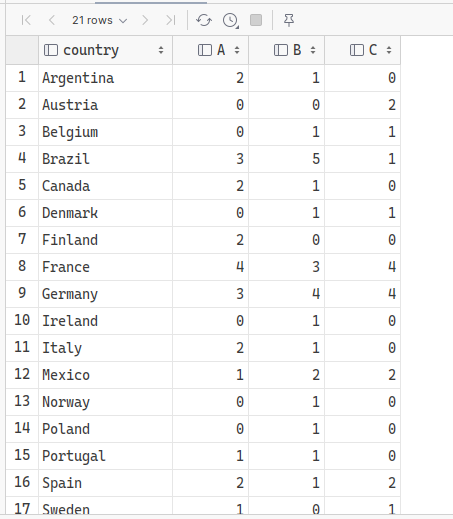
\includegraphics[width=0.8\textwidth]{./images/5.png}
        \end{center}
    }
    \pagebreak
    \item {
        Apakah hasilnya sama persis dengan hasil yang ada pada Praktikum Bagian 1?
        Mengapa demikian?

        Hal ini dikarenakan query hanya mengubah subquery menjadi common table expression (CTE).
    }
    \item {
        Apakah keuntungan penggunaan CTE ketika membuat query yang menggunakan
        operator PIVOT?

        Query dapat menjadi lebih ringkas karena tidak perlu menuliskan subquery lagi sehingga
        query terlihat lebih rapi.
    }
    \pagebreak
    \item {
        Buatlah sebuah query SELECT yang menampilkan data total jumlah penjualan untuk
        setiap kategori produk, untuk setiap customer. Tampilkan setiap kategori produk ke dalam
        kolom tersendiri, seperti pada tampilan di bawah ini.

        \begin{minted}[autogobble,fontsize=\small]{sql}
            SELECT
                custid,
                [Beverages],
                [Condiments],
                [Confections],
                [Dairy Products],
                [Grains/Cereals],
                [Meat/Poultry],
                [Produce],
                [Seafood]
            FROM (
                SELECT * FROM SalesByCategory
            ) as SourceTable
            PIVOT (
                SUM(SalesValue)
                FOR categoryname IN (
                    [Beverages],
                    [Condiments],
                    [Confections],
                    [Dairy Products],
                    [Grains/Cereals],
                    [Meat/Poultry],
                    [Produce],
                    [Seafood]
                )
            ) as PivotTable;
        \end{minted}

        \begin{center}
            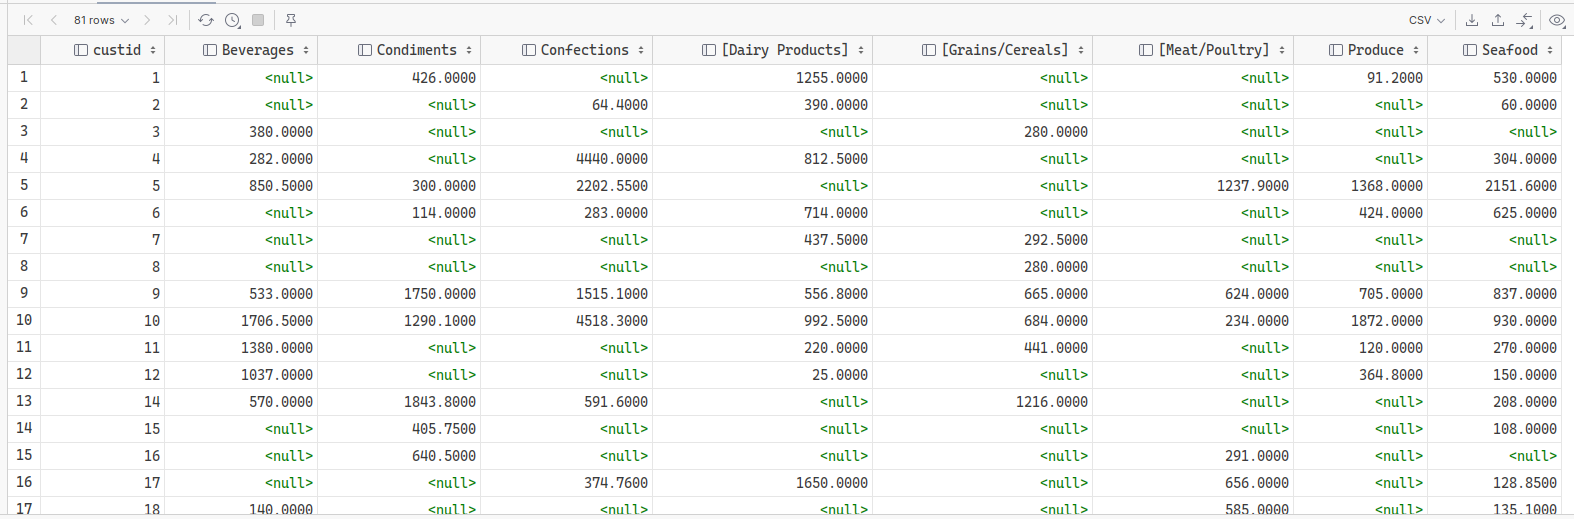
\includegraphics[width=0.8\textwidth]{./images/8.png}
        \end{center}
    }
    \pagebreak
    \item {
        Buatlah query SELECT yang menghasilkan kolom country, kolom A, kolom B, dan kolom
        C dari view Sales.PivotCustGroups yang telah dibuat.

        \begin{minted}[autogobble,fontsize=\small]{sql}
            SELECT country, A, B, C
            FROM Sales.PivotCustGroups;
        \end{minted}

        \begin{center}
            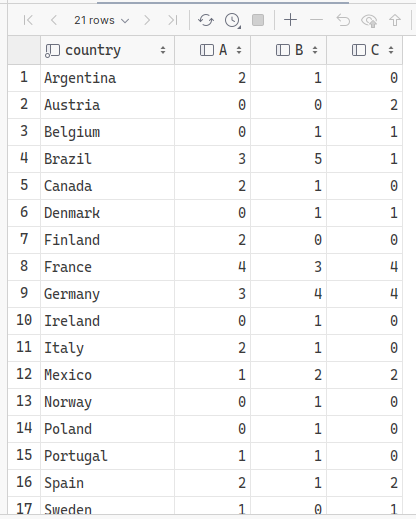
\includegraphics[width=0.8\textwidth]{./images/9.png}
        \end{center}
    }
    \pagebreak
    \item {
        Buatlah sebuah query SELECT terhadap view Sales.PivotCustGroups yang
        menghasilkan data seperti tampilan berikut: 

        \begin{minted}[autogobble,fontsize=\small]{sql}
            SELECT custgroup, country, SUM(numberofcustomers) AS numberofcustomers
            FROM Sales.PivotCustGroups
            UNPIVOT (
                numberofcustomers
                FOR custgroup IN (
                    A, B, C
                )
            ) AS unpivoted
            GROUP BY custgroup, country
            ORDER BY country;
        \end{minted}

        \begin{center}
            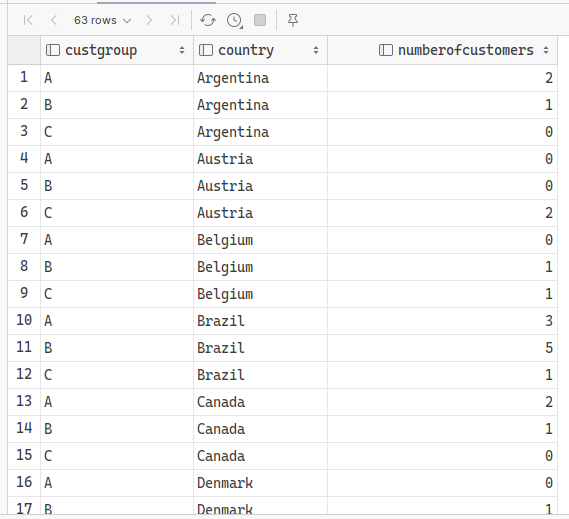
\includegraphics[width=0.8\textwidth]{./images/10.png}
        \end{center}
    }
    \pagebreak
    \item {
        Buatlah query SELECT terhadap tabel Sales.Customers yang terdiri dari kolom contry,
        city, dan kolom kalkulasi yang menghitung banyaknya customer bernama noofcustomers.
        Dapatkan pengelompokan (grouping set) berdasarkan:
        \begin{itemize}
            \item kolom country dan city
            \item kolom country
            \item kolom city
            \item dan sebuah kolom tanpa kelompok 
        \end{itemize}

        \begin{minted}[autogobble,fontsize=\small]{sql}
            SELECT country, city, COUNT(*) AS noofcustomers
            FROM Sales.Customers
            GROUP BY GROUPING SETS (
                (country, city),
                (country),
                (city),
                ()
            );
        \end{minted}

        \begin{center}
            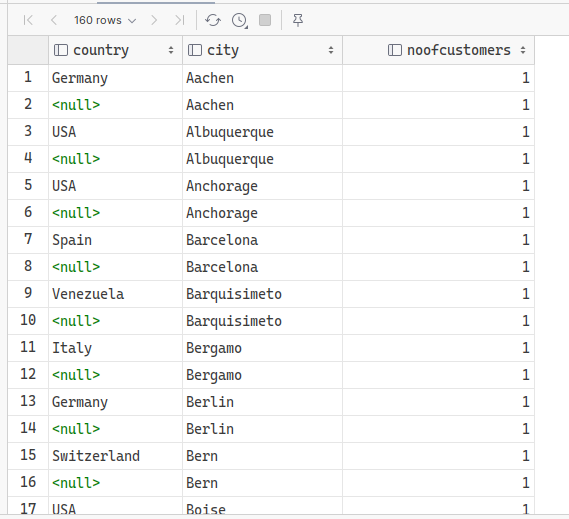
\includegraphics[width=0.8\textwidth]{./images/11.png}
        \end{center}
    }
    \pagebreak
    \item {
        Buatlah sebuah query SELECT terhadap view Sales.OrderValues yang berisi kolom:
        \begin{itemize}
            \item \texttt{orderyear}: tahun dari kolom orderdate
            \item \texttt{ordermounth}: bulan dari kolom orderdate
            \item \texttt{orderday}: hari dari kolom orderdate
            \item \texttt{salesvalue}: total jumlah penjualan dari kolom val
        \end{itemize}

        \begin{minted}[autogobble,fontsize=\small]{sql}
            SELECT 
                YEAR(orderdate) AS orderyear,
                MONTH(orderdate) AS ordermonth,
                DAY(orderdate) AS orderday,
                SUM(val) AS salesvalue
            FROM Sales.OrderValues
            GROUP BY CUBE (
                YEAR(orderdate),
                MONTH(orderdate),
                DAY(orderdate)
            );
        \end{minted}

        \begin{center}
            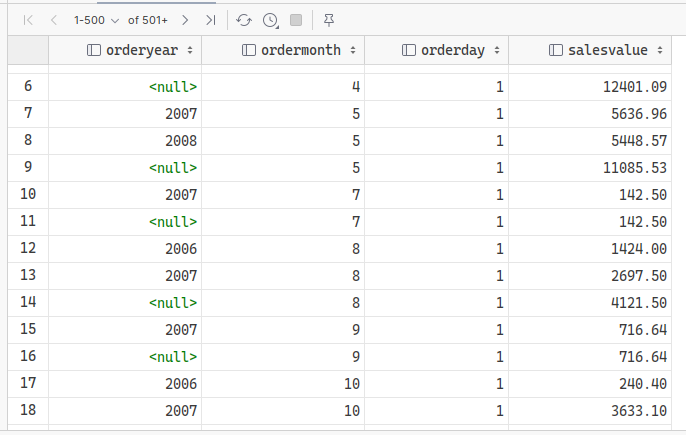
\includegraphics[width=0.8\textwidth]{./images/12.png}
        \end{center}
    }
    \pagebreak
    \item {
        Salinlah query dari Soal no 12 di atas dan ubah sub klausa CUBE menjadi ROLLUP, lalu
        jalankan query tersebut.

        \begin{minted}[autogobble,fontsize=\small]{sql}
            SELECT 
                YEAR(orderdate) AS orderyear,
                MONTH(orderdate) AS ordermonth,
                DAY(orderdate) AS orderday,
                SUM(val) AS salesvalue
            FROM Sales.OrderValues
            GROUP BY ROLLUP (
                YEAR(orderdate),
                MONTH(orderdate),
                DAY(orderdate)
            );
        \end{minted}

        \begin{center}
            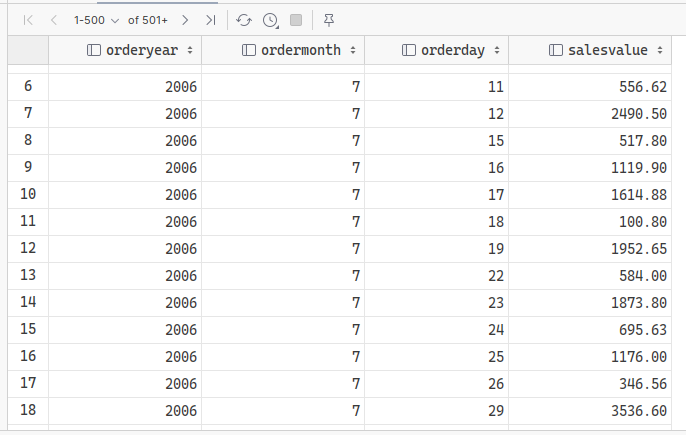
\includegraphics[width=0.8\textwidth]{./images/13.png}
        \end{center}
    }
    \pagebreak
    \item {
        Apakah perbedaan antara sub klausa ROLLUP dan CUBE? Manakah yang lebih tepat
        digunakan untuk query pada langkah 1 di atas?

        Perbedaan antara sub klausa ROLLUP dan CUBE adalah ROLLUP hanya menghasilkan subtotal
        untuk kolom yang ditentukan sedangkan CUBE menghasilkan subtotal untuk semua kolom.
    }
    \pagebreak
    \item {
        Buatlah query SELECT terhadap view Sales.OrderValues dan dapatkan kolom berikut
        ini:
        \begin{itemize}
            \item kolom kalkulasi dengan nama alias groupid (gunakan fungsi GROUPING\_ID dengan tahun order dan bulan order sebagai parameter inputnya)
            \item orderyear: tahun dari kolom orderdate
            \item ordermonth: bulan dari kolom orderdate
            \item salesvalue: total nilai penjualan dari kolom val
            \item oleh karena tahun dan bulan berbentuk hierarki, dapatkan semua pengelompokan/ grouping set berdasarkan kolom orderyear dan ordermonth, lalu urutkan berdasarkan groupid, orderyear, dan ordermonth
        \end{itemize}

        \begin{minted}[autogobble,fontsize=\small]{sql}
            SELECT
                GROUPING_ID(YEAR(orderdate),
                MONTH(orderdate)) AS groupid,
                YEAR(orderdate) AS orderyear,
                MONTH(orderdate) AS ordermonth,
                SUM(val) AS salesvalue
            FROM Sales.OrderValues
            GROUP BY ROLLUP (
                YEAR(orderdate),
                MONTH(orderdate)
            )
            ORDER BY groupid, orderyear, ordermonth;
        \end{minted}

        \begin{center}
            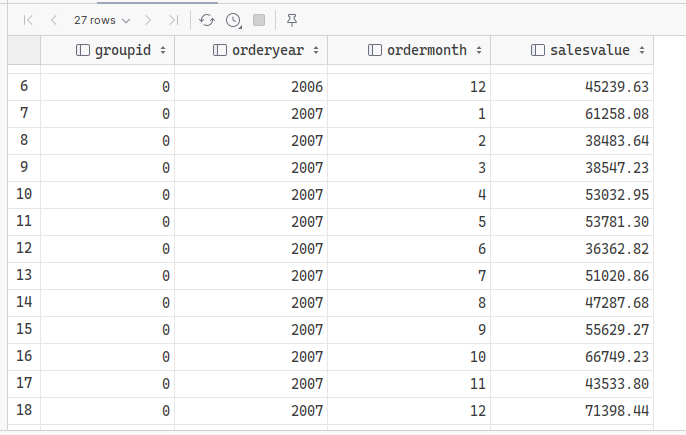
\includegraphics[width=0.8\textwidth]{./images/15.png}
        \end{center}
    }
    \end{enumerate}
\end{document}

